\documentclass[a4paper,11pt,dvipdfmx]{ujarticle}
% パッケージ
\usepackage{graphicx}
\usepackage{url}
% レイアウト指定を記述したファイルの読み込み
\input{layout}

% タイトルと氏名を変更せよ.
\title{日本におけるデジタル化の状況}
\author{G584202025 伊田 大輝}

\begin{document}

\maketitle

\section{ブローバンドの整備状況}

OECDによるブローバンド回線の普及に関する調査\cite{oecd}によると、図1に示すように、
日本における100人あたりのモバイルブローバンドの加入者数は190.5で、
第1位になっている。2位はエストニアで、3位米国と続く。

% 節見出し: \section{}
% を使う

% 本文(1)

% を使う
% 文献データベースのキーワードは oecd と imd
% になっている.

\begin{figure}[htbp]
    \centering
    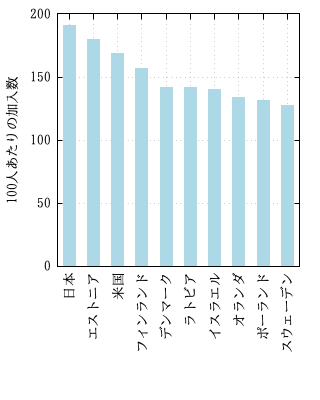
\includegraphics{abc.png}
    \caption{光ファイバー回線の加入者数(100人あたり)}\label{図1}
\end{figure}
% ーーー
\section{デジタル競争力ランキング}

国際経営研究所(IMD)の調査\cite{imd}によると、日本のデジタル競争力ランキングは表1
に示すように、調査対象の64カ国中、総合で28位、準備分野で27位となっている。

\begin{table}[htbp]
    \centering
    \caption{デジタル競争力ランキング(64カ国中)}\label{表1}
    \begin{tabular}{|c|c|c|}
        \hline
        国 & 総合 & 準備 \\
        \hline
        米国 & 1位 & 1位 \\
        \hline
        香港 & 2位 & 10位 \\
        \hline
        スウェーデン & 3位 & 6位 \\
        \hline
        デンマーク & 4位 & 2位 \\
        \hline
        シンガポール & 5位 & 11位 \\
        \hline
        \hline
            韓国    & 12位 & 5位 \\
        \hline
            中国    & 15位 & 17位 \\
        \hline
        \hline
        日本 & 28位 & 27位 \\
        \hline
    \end{tabular}
\end{table}
% を使って表番号が参照できるようにする
% また,
% で表が中央に来るようにする
% ーーー
% 見出し(3)
\section{考察}
\begin{itemize}
    \item{日本はインフラが整っているがリスク回避志向が強く、
    新規事業やIT活用に積極的でない企業が多いため、
    デジタル化の進展が遅れる。}
    \item{現在の日本はIT人材が不足していて、
    教育や研修も追いついていないので、
    新しい技術の普及が進みにくい}
    \item{通信インフラの普及率はあまり
    競争力には繋がらない}
\end{itemize}
% を使って箇条書きで記述する

\bibliographystyle{junsrt}
\bibliography{exercise.bib}

\end{document}